\chapter*{Findings}
\label{sec:Insecure coding}
\begin{table}[htb]
    \renewcommand{\arraystretch}{1.5}
    \begin{tabular*}{\textwidth}{|>{\columncolor{orange!15}}p{3cm}|p{17.1cm}|}
    \textbf{Finding} & \textbf{Insecure coding leads to disk-image access}\\
    Risk& Low\\
    Category& Obfuscation, information disclosure\\
    Impact& An attacker can obtain the passphrase to decrypt the disk-image file 'container.img'\\\\ 
    Description& Analyzing the file system of the server named 'plunder' running on port 22, a disk-image file 'container.img' was found. After trying to mount the image the following error message appeared:
    \newline
    \newline
    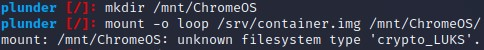
\includegraphics{mount_error.jpg}
    \newline
    \newline
    Given that the filesystem is apparently from type 'crypto\_LUKS' the disk-image is most likely encrypted. Through research the following command was tried to decrypt the filesystem:
    \newline
    \newline
    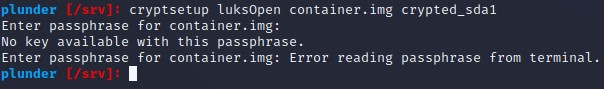
\includegraphics{cryptsetup_enterpassphrase.jpg}
    \newline
    \newline
    The first method to access the container image was a brute force attack. Since we have credentials for the SSH we copied the image to our local kali linux machine with the following command: ''scp root@172.16.0.29:/srv/container.img output.img''
    After copying the file a brute force attack was performed using the tool bruteforce-luks.
    \newline
    \newline
    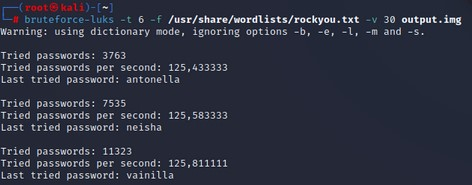
\includegraphics{brute-force-luks.jpg}
    \newline
    \newline
    However there was no matching password found with this method.   
    \end{tabular*}
    \end{table}